\documentclass[12pt]{article}
\usepackage{graphicx}
\usepackage{amsmath,amssymb}

\renewcommand{\baselinestretch}{2}
\setlength{\parindent}{0pt}
\setlength{\parskip}{0.75\baselineskip}

\makeatletter
\long\def\@makecaption#1#2{%
    \vskip\abovecaptionskip
    \small
    \sbox\@tempboxa{#1. #2}%
    \ifdim \wd\@tempboxa >\hsize
        #1. #2\par
    \else
        \global \@minipagefalse
        \hb@xt@\hsize{\hfil\box\@tempboxa\hfil}%
    \fi
    \vskip\belowcaptionskip}
\makeatother

\title{Tail Risk in SPY and XLF: GJR-GARCH vs EGARCH}
\author{Ruiwen He}
\date{\today}

\begin{document}
\maketitle

\begin{abstract}
This report evaluates asymmetric volatility models for tail-risk management using daily log returns of SPY and XLF from 2016-01-01 to 2026-01-01. Two models, GJR-GARCH(1,1) and EGARCH(1,1), are estimated on an in-sample period (80\%) and assessed by rolling one-step-ahead out-of-sample forecasts (20\%). Dynamic Value-at-Risk (VaR) and Expected Shortfall (ES) are computed at 95\% and 99\% confidence levels under Normal innovations, followed by exception-rate backtesting. The evidence shows strong volatility clustering, negative skewness, and heavy tails in both assets. At the extreme 99\% confidence level, GJR-GARCH delivers tighter exception-rate alignment than EGARCH for both SPY and XLF, indicating more reliable tail coverage in severe market conditions.\end{abstract}

\section{Introduction \& Executive Summary}
Tail-risk management is central to financial institutions because solvency stress is driven by low-probability, high-impact losses rather than average market fluctuations. In practice, volatility is time-varying and clustered; moreover, downside shocks typically generate larger volatility responses than upside shocks of similar magnitude. This asymmetry, commonly referred to as the leverage effect, is critical for market-risk systems that must remain robust during crisis regimes.

The asset selection is intentionally macro-to-sectoral. SPY (S\&P 500 ETF) proxies broad U.S. market risk and captures the aggregate macro-financial state. XLF (Financial Select Sector SPDR Fund) concentrates exposure to banks and diversified financial institutions, a segment with strong procyclicality, balance-sheet sensitivity, and systemic relevance. Comparing SPY and XLF therefore reveals whether asymmetric volatility models scale consistently from broad market risk to a shock-amplifying sector.

The key business conclusion is straightforward. Both models fit the data well, but under the stricter 99\% tail standard used in supervisory and internal stress governance, GJR-GARCH produces better calibrated exception rates than EGARCH for both SPY and XLF in the out-of-sample period. This makes GJR-GARCH the preferred baseline for extreme-loss monitoring in this sample, while EGARCH remains competitive for in-sample fit metrics and 95\% coverage in selected cases.

\section{Theoretical Framework}
\subsection{Return and Error Decomposition}
Let daily return be
\begin{equation}
    r_t = \mu_t + \epsilon_t,
\end{equation}
with innovation
\begin{equation}
    \epsilon_t = \sigma_t z_t,
\end{equation}
where $\sigma_t$ is conditional volatility and $z_t$ is an i.i.d. standardized shock. Under baseline assumptions, $z_t \sim \mathcal{N}(0,1)$; a Student-$t$ alternative can be used to model heavier tails.

\subsection{GJR-GARCH(1,1)}
The GJR-GARCH variance recursion is
\begin{equation}
    \sigma_t^2 = \omega + (\alpha + \gamma I_{t-1})\epsilon_{t-1}^2 + \beta\sigma_{t-1}^2,
\end{equation}
where
\begin{equation}
    I_{t-1} = \begin{cases}
        1, & \text{if } r_{t-1} < 0,\\
        0, & \text{if } r_{t-1} \ge 0.
    \end{cases}
\end{equation}
Interpretation is immediate. For positive-return days, the shock-loading term is $\alpha$; for negative-return days, it is $\alpha + \gamma$. A positive and significant $\gamma$ quantifies a stronger volatility response to bad news and operationalizes downside asymmetry.

\subsection{EGARCH(1,1)}
The EGARCH specification is
\begin{equation}
\ln(\sigma_t^2)=\omega + \alpha\left(|z_{t-1}|-\mathbb{E}|z_{t-1}|\right)+\gamma z_{t-1}+\beta\ln(\sigma_{t-1}^2).
\end{equation}
Because the model evolves in log-variance space, positivity of $\sigma_t^2$ is guaranteed without imposing non-negativity constraints on ARCH coefficients. The signed term $\gamma z_{t-1}$ captures directional asymmetry: when $\gamma<0$, negative shocks increase volatility more than positive shocks.

\subsection{Dynamic VaR and ES}
For left-tail risk at confidence level $c \in \{0.95,0.99\}$, define tail probability $\alpha=1-c$. Let $q_\alpha$ denote the $\alpha$-quantile of $z_t$. Then one-step-ahead conditional VaR is
\begin{equation}
\mathrm{VaR}_{c,t+1}=\mu_{t+1}+\sigma_{t+1}q_\alpha.
\end{equation}
For Normal innovations, $q_\alpha=\Phi^{-1}(\alpha)$.

Expected Shortfall is the conditional expectation beyond VaR:
\begin{equation}
\mathrm{ES}_{c,t+1}=\mathbb{E}\left[r_{t+1}\mid r_{t+1}\le \mathrm{VaR}_{c,t+1}\right].
\end{equation}
Under Normality,
\begin{equation}
\mathrm{ES}_{c,t+1}=\mu_{t+1}-\sigma_{t+1}\frac{\phi\left(\Phi^{-1}(\alpha)\right)}{\alpha},
\end{equation}
where $\phi(\cdot)$ and $\Phi(\cdot)$ are the standard Normal pdf and cdf. In implementation, $\mu_{t+1}$ is set to zero for conservative and stable short-horizon risk forecasting.

\section{Data \& Exploratory Data Analysis}
\subsection{Sample and Construction}
The dataset contains daily log returns (in percentage points) for SPY and XLF from 2016-01-01 to 2026-01-01, totaling 2,513 observations per series. Prices are downloaded via Yahoo Finance and transformed as
\begin{equation}
    r_t = 100\times\left(\ln P_t - \ln P_{t-1}\right).
\end{equation}
The sample includes two major stress windows highlighted in the time-series plot: the COVID shock (March 2020) and the U.S. regional banking stress episode around Silicon Valley Bank (March 2023).

\subsection{Descriptive Statistics}
Table~\ref{tab:desc} confirms non-Gaussian return behavior: both assets are negatively skewed and strongly leptokurtic.

\begin{table}[htbp]
\centering
\caption{Descriptive Statistics of Daily Log Returns (\%)}
\label{tab:desc}
\begin{tabular}{lrrrrrrr}
\hline
Asset & Mean & Std & Skewness & Kurtosis & Min & Max & Obs \\
\hline
SPY & 0.0552 & 1.1369 & -0.6048 & 18.1541 & -11.5887 & 9.9863 & 2513 \\
XLF & 0.0496 & 1.4087 & -0.5880 & 18.5290 & -14.7448 & 12.3602 & 2513 \\
\hline
\end{tabular}
\end{table}

XLF exhibits higher volatility and deeper downside realizations than SPY, consistent with stronger cyclicality and higher crisis sensitivity in the financial sector.

\begin{figure}[htbp]
\centering
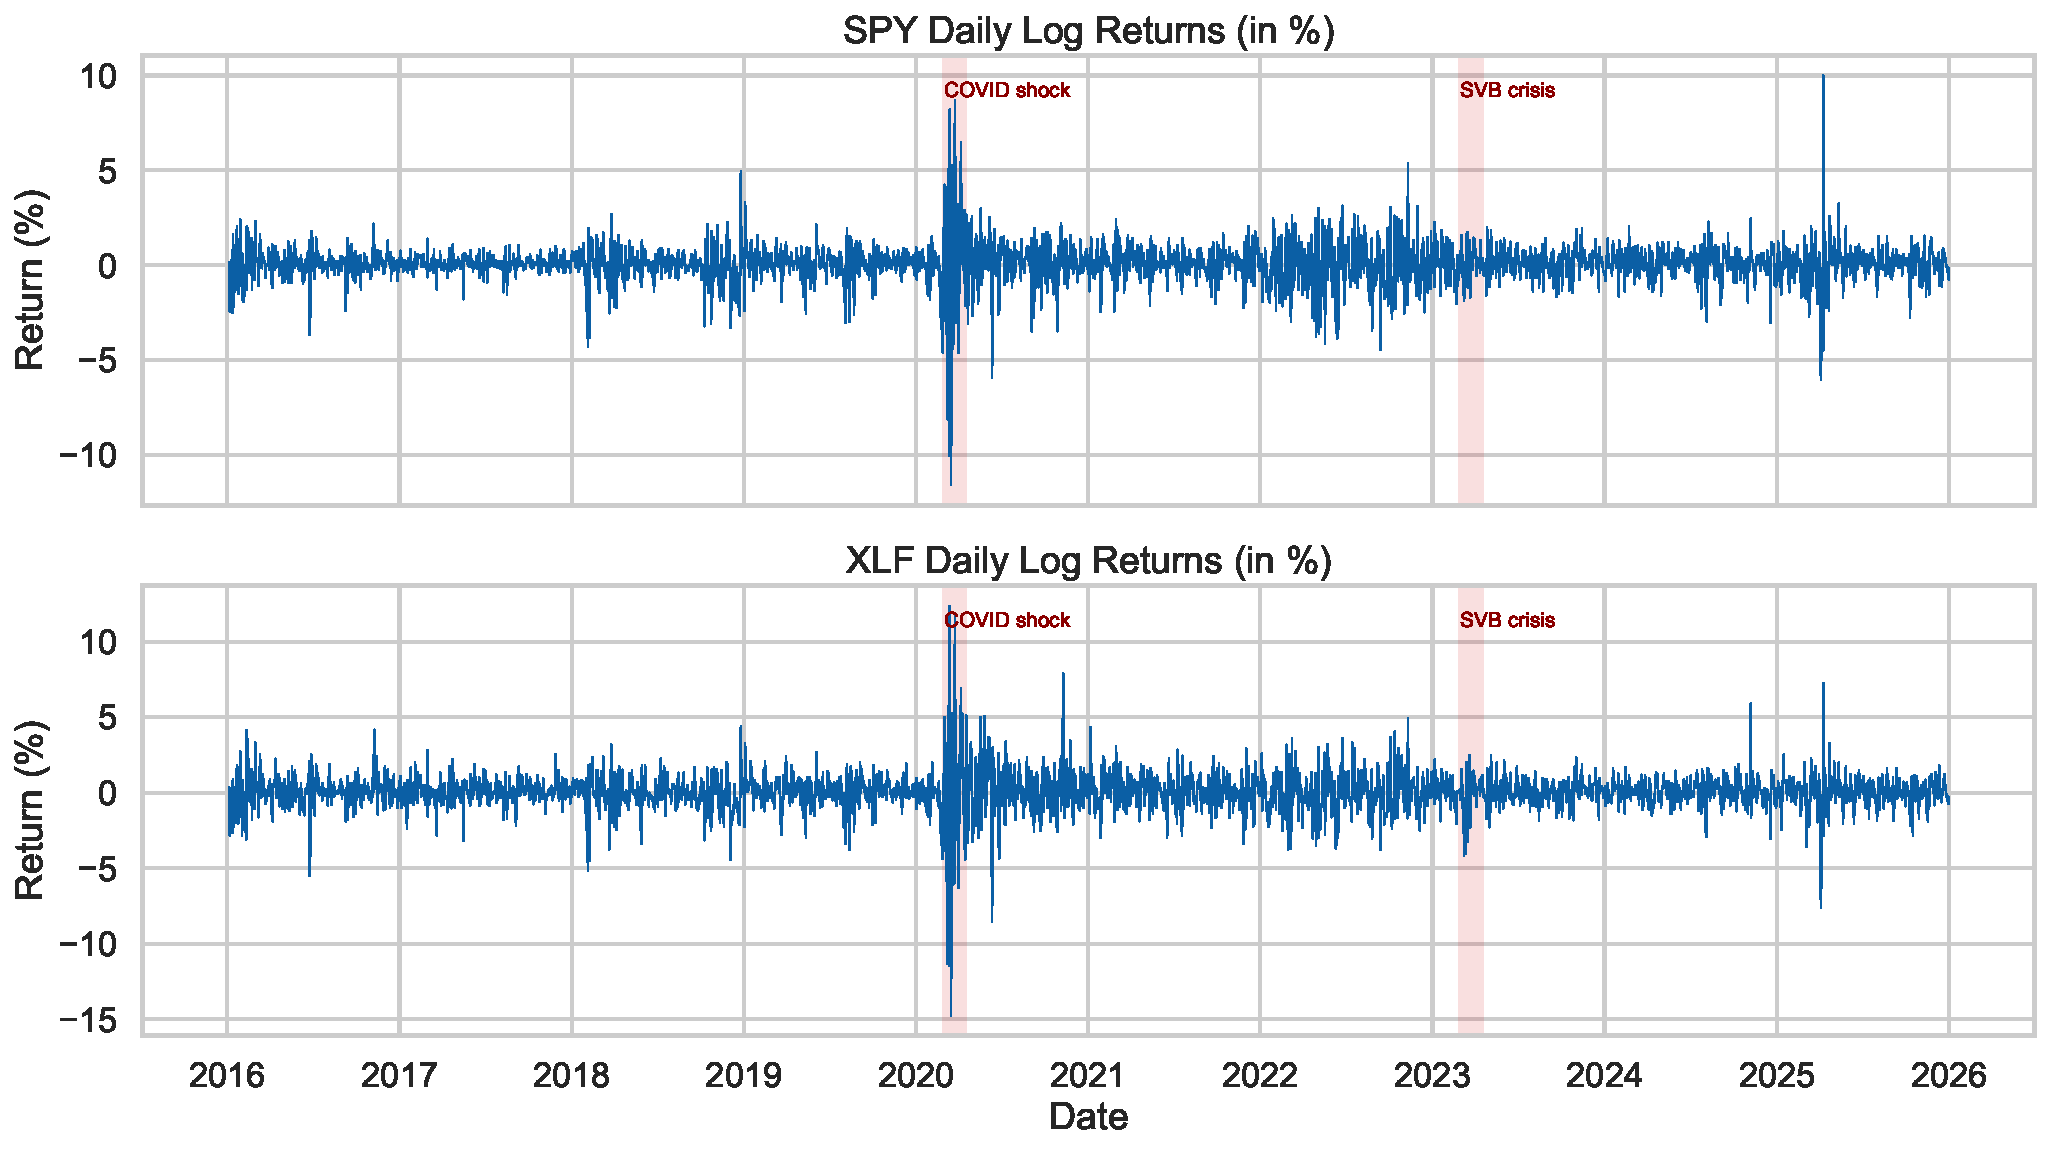
\includegraphics[width=0.95\textwidth]{outputs/figures/figure1_returns_with_stress_periods.pdf}
\caption{SPY and XLF Daily Returns with Highlighted Stress Periods (COVID 2020 and SVB 2023).}
\label{fig:returns}
\end{figure}

\section{Empirical Results \& Model Estimation}
\subsection{In-Sample Estimation Design}
The first 80\% of observations (roughly 2016 through end-2023) are used for parameter estimation. Both GJR-GARCH(1,1) and EGARCH(1,1) are estimated with Normal innovations using maximum likelihood.

\subsection{Key Parameter Evidence}
The asymmetric terms are statistically significant in all specifications. For GJR-GARCH, the leverage parameter is positive and highly significant for both assets: $\gamma_{\text{SPY}}=0.2002$ ($p<0.001$) and $\gamma_{\text{XLF}}=0.2024$ ($p<0.001$). For EGARCH, the signed asymmetry term is negative and highly significant: $\gamma_{\text{SPY}}=-0.1448$ and $\gamma_{\text{XLF}}=-0.1365$, both with very small $p$-values.

These estimates provide robust evidence of bad-news amplification. XLF shows at least comparable and often stronger asymmetry significance than SPY, consistent with the economic narrative that financial stocks react more sharply under downside stress.

\subsection{Information Criteria Comparison}
Table~\ref{tab:ic} reports in-sample fit diagnostics.

\begin{table}[htbp]
\centering
\caption{Information Criteria by Asset and Model (In-Sample)}
\label{tab:ic}
\begin{tabular}{llrrr}
\hline
Ticker & Model & AIC & BIC & LogLik \\
\hline
SPY & GJR-GARCH & 5146.0073 & 5174.0368 & -2568.0037 \\
SPY & EGARCH & 5128.8780 & 5156.9075 & -2559.4390 \\
XLF & GJR-GARCH & 6343.1126 & 6371.1420 & -3166.5563 \\
XLF & EGARCH & 6341.6990 & 6369.7285 & -3165.8495 \\
\hline
\end{tabular}
\end{table}

EGARCH provides slightly lower AIC/BIC for both assets, indicating marginally better in-sample likelihood fit.

\section{Risk Management Application: VaR \& ES}
\subsection{Out-of-Sample Rolling Forecast Setup}
The last 20\% of observations (approximately 2024--2025) are reserved for out-of-sample evaluation. A one-step-ahead fixed-window rolling procedure generates time-varying volatility forecasts $\hat{\sigma}_{t+1}$ and corresponding dynamic VaR/ES at 95\% and 99\%.

\subsection{Dynamic Risk Boundary Behavior}
Figure~\ref{fig:var_spy_gjr} illustrates the expected risk-system behavior: during high-volatility episodes, the estimated lower-tail VaR bands move downward (become more conservative), widening the protective buffer against large losses.

\begin{figure}[htbp]
\centering
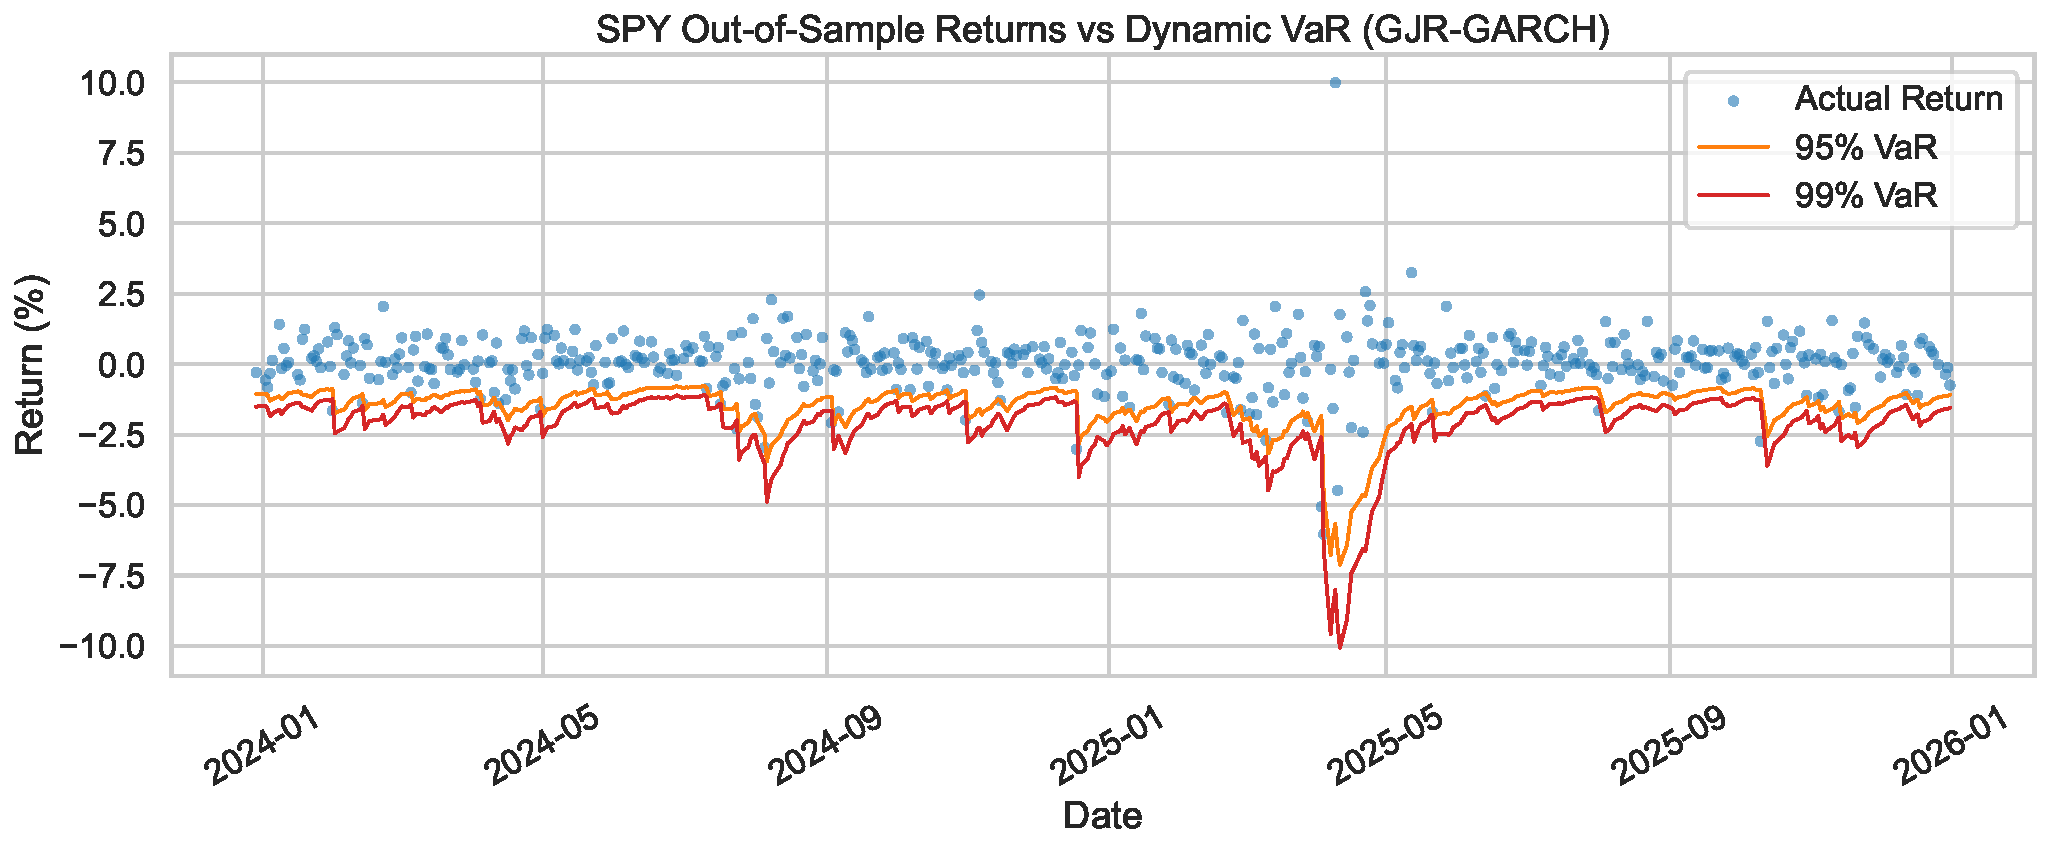
\includegraphics[width=0.95\textwidth]{outputs/figures/figure2_var_overlay_SPY_GJR-GARCH.pdf}
\caption{SPY Out-of-Sample Returns with Dynamic 95\% and 99\% VaR (GJR-GARCH).}
\label{fig:var_spy_gjr}
\end{figure}

To explicitly incorporate tail severity (not only tail quantiles), Figure~\ref{fig:var_es_spy_gjr} overlays ES alongside VaR. As expected, ES is always more conservative (more negative) than VaR at the same confidence level, and the ES bands widen further during volatility bursts.

\begin{figure}[htbp]
\centering
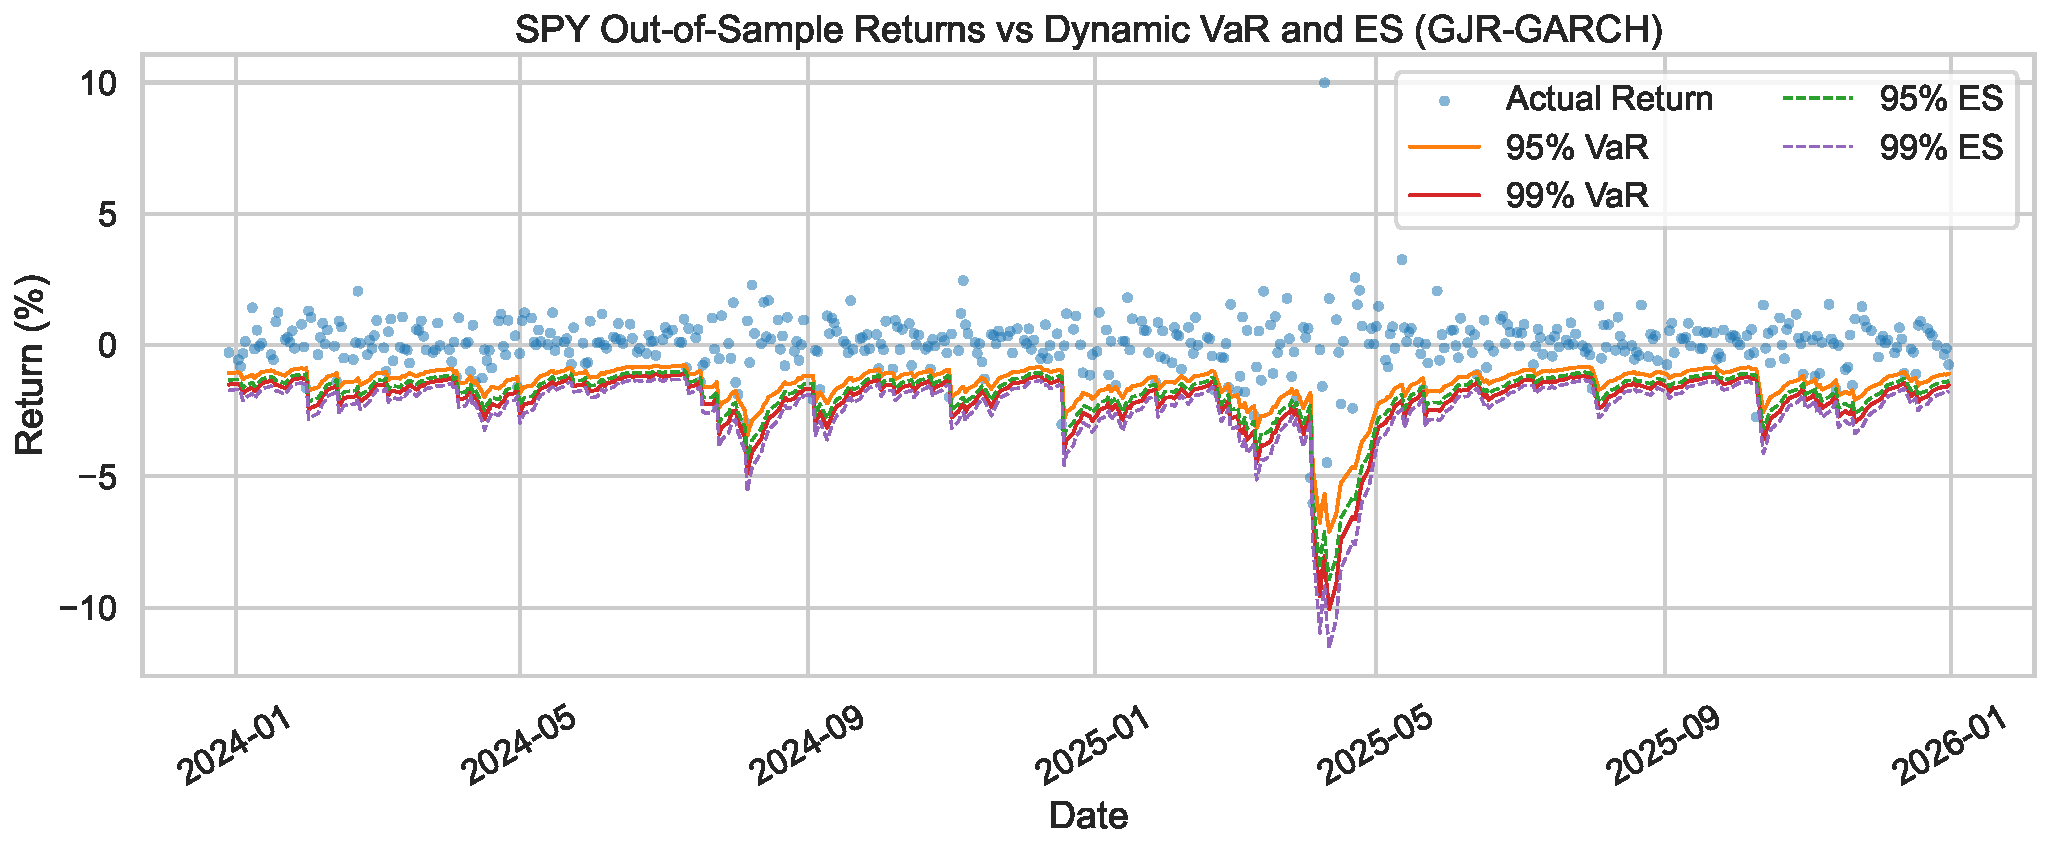
\includegraphics[width=0.95\textwidth]{outputs/figures/figure3_var_es_overlay_SPY_GJR-GARCH.pdf}
\caption{SPY Out-of-Sample Returns with Dynamic VaR and ES (GJR-GARCH).}
\label{fig:var_es_spy_gjr}
\end{figure}

\subsection{Backtesting via Exceptions}
Table~\ref{tab:bt} compares observed versus expected exception frequencies.

\begin{table}[htbp]
\centering
\caption{VaR Exception Backtesting Summary (Out-of-Sample)}
\label{tab:bt}
\begin{tabular}{llrrrr}
\hline
Ticker & Model & VaR Level & Expected Rate & Observed Rate & Abs. Error \\
\hline
SPY & GJR-GARCH & 95\% & 0.0500 & 0.0497 & 0.0003 \\
SPY & GJR-GARCH & 99\% & 0.0100 & 0.0199 & 0.0099 \\
SPY & EGARCH & 95\% & 0.0500 & 0.0497 & 0.0003 \\
SPY & EGARCH & 99\% & 0.0100 & 0.0239 & 0.0139 \\
XLF & GJR-GARCH & 95\% & 0.0500 & 0.0378 & 0.0122 \\
XLF & GJR-GARCH & 99\% & 0.0100 & 0.0179 & 0.0079 \\
XLF & EGARCH & 95\% & 0.0500 & 0.0457 & 0.0043 \\
XLF & EGARCH & 99\% & 0.0100 & 0.0199 & 0.0099 \\
\hline
\end{tabular}
\end{table}

At 99\%, GJR-GARCH has lower absolute calibration error than EGARCH for both SPY and XLF, which is operationally important for stress-capital decisions and downside limit setting. At 95\%, SPY is effectively tied across models while EGARCH performs better for XLF.

\subsection{ES Backtesting and Tail-Loss Accuracy}
ES is assessed on VaR-breach days by comparing realized tail mean losses against the model-implied ES mean. Table~\ref{tab:esbt} reports the gap
\begin{equation}
\text{ES Gap} = \overline{r_t\mid r_t<\mathrm{VaR}} - \overline{\mathrm{ES}_t\mid r_t<\mathrm{VaR}}.
\end{equation}
Values below zero indicate realized losses are more severe than predicted ES (underestimation of tail severity).

\begin{table}[htbp]
\centering
\caption{ES Backtesting Summary on VaR-Breach Days (Out-of-Sample)}
\label{tab:esbt}
\begin{tabular}{llrrrr}
\hline
Ticker & Model & ES Level & Tail Obs & Realized Tail Mean & Predicted ES Mean \\
\hline
SPY & GJR-GARCH & 95\% & 25 & -2.0963 & -1.7581 \\
SPY & GJR-GARCH & 99\% & 10 & -2.3606 & -1.7891 \\
SPY & EGARCH & 95\% & 25 & -2.0963 & -1.7623 \\
SPY & EGARCH & 99\% & 12 & -2.6115 & -2.2433 \\
XLF & GJR-GARCH & 95\% & 19 & -2.6258 & -2.1766 \\
XLF & GJR-GARCH & 99\% & 9 & -3.4286 & -3.0286 \\
XLF & EGARCH & 95\% & 23 & -2.3819 & -2.0181 \\
XLF & EGARCH & 99\% & 10 & -3.2706 & -2.8414 \\
\hline
\end{tabular}
\end{table}

The ES results indicate that both models underestimate extreme tail severity on breach days (all ES gaps are negative). In relative terms, EGARCH is slightly closer at SPY 99\% and XLF 95\%, while GJR-GARCH is closer at SPY 95\% and XLF 99\%. Combined with VaR exception calibration, this suggests a practical hybrid interpretation: GJR-GARCH is preferable for 99\% quantile control, whereas ES severity diagnostics should still be monitored model-by-model.

\section{Conclusion}
This study compares GJR-GARCH and EGARCH for dynamic market-risk measurement in SPY and XLF. Three conclusions emerge. First, both assets display strong non-normality and asymmetric volatility dynamics, validating the use of asymmetric conditional-variance models. Second, EGARCH slightly dominates in-sample information criteria. Third, and most relevant for risk governance, GJR-GARCH provides better 99\% VaR calibration in out-of-sample backtesting for both assets.

For practical deployment, institutions should prioritize model performance at extreme confidence levels and complement VaR with ES for tail severity control. In Basel-oriented settings and banking-sector stress regimes, 99\% ES offers a more conservative and policy-aligned safety layer than standalone 95\% VaR thresholds.

\section{Appendix: Replication Instructions}
\subsection*{Environment}
Python 3.11 in Conda environment \texttt{myenv}. Core packages:
\texttt{pandas, numpy, yfinance, arch, scipy, matplotlib, seaborn}.

\subsection*{Project Files}
Current implementation is script-centric:
\begin{itemize}
    \item \texttt{codes.py}: full pipeline (download, estimation, forecasting, VaR/ES, plotting, exports)
    \item \texttt{outputs/data}: return and VaR/ES time-series CSV files
    \item \texttt{outputs/tables}: descriptive, estimation, IC, and backtesting tables
    \item \texttt{outputs/tables/es\_backtest\_summary.csv}: ES tail-loss evaluation table
    \item \texttt{outputs/figures}: Figure 1, VaR overlays (Figure 2), and VaR+ES overlays (Figure 3)
\end{itemize}

\subsection*{Reproducibility and Execution Guide}
\begin{enumerate}
    \item Go to the project folder: \texttt{Assignment Answers by Ruiwen HE/FINAL PAPER}.
    \item Run the full pipeline:
\begin{verbatim}
D:/Programming/Python/Conda/envs/myenv/python.exe codes.py
\end{verbatim}
    \item Review generated artifacts in:\\
    \texttt{outputs/data} (time-series data), \texttt{outputs/tables} (empirical tables), and \texttt{outputs/figures} (publication figures).
\end{enumerate}

\end{document}
